\documentclass[conference]{IEEEtran}

\usepackage{cite}
\usepackage{amsmath}
\usepackage{url}
\usepackage{hyperref}
\hypersetup{hidelinks}
\usepackage{booktabs}
\usepackage{multirow}
\usepackage{graphicx}
\usepackage{listings}
\usepackage[table]{xcolor}
\usepackage{tikz}
\usepackage{flushend}
\usetikzlibrary{arrows.meta,positioning,shapes.geometric}

\lstdefinestyle{prompt}{
  basicstyle=\ttfamily\footnotesize,
  breaklines=true,
  columns=fullflexible,
  frame=single,
  framerule=0.3pt,
  xleftmargin=0.8em,
  xrightmargin=0.8em,
  aboveskip=0.6em,
  belowskip=0.6em,
  showstringspaces=false
}

\title{Reproducing and Extending TISER:\\
Context--Memory Conflict and Tennis-Domain Adaptation for Temporal Reasoning}

\author{
\IEEEauthorblockN{
Gabriele Adorni s349308,
Alessandro Casadei s349386, \\
Taha Atabay Cetin s349501
}
\IEEEauthorblockA{
Politecnico di Torino\\
Deep Natural Language Processing
}
}

\begin{document}

\maketitle

\begin{abstract}
Temporal reasoning requires a model to organise events before answering questions about order, duration, and overlap. We reproduce TISER, a framework that elicits a structured reasoning trace with an explicit timeline and reflection step, and evaluate two extensions with different goals. First, an inference-time Context--Memory Conflict probe tests whether a model follows supplied evidence when it contradicts a fact the model recalls without context. Second, a supervised tennis-domain study tests whether TISER transfers to a new type of temporal narrative and whether further adaptation helps. The reproduction reaches macro exact match of 0.878 and macro F1 of 0.949 on five in-domain benchmarks. On 1,056 genuine conflict cases, combining the TISER-trained model and prompt raises context-faithful exact match from 0.348 to 0.774, although explicit conflict detection remains rare and order reversals remain difficult. On tennis questions, direct transfer reaches exact match of 0.580; continued adaptation increases it to 0.732. These results distinguish grounded use of context from explicit self-auditing and show that temporal-reasoning behaviour can transfer across domains.
\end{abstract}

\section{Introduction}

Temporal reasoning---interpreting event order, overlap, and duration---is central to question answering and narrative understanding. Large language models often identify the relevant events yet misalign them in time, confuse start and end points, or return a semantically correct answer in a form that exact-match metrics reject.

TISER~\cite{bazaga2025tiser} addresses this problem by training a model to produce four tagged stages before its final response: \texttt{<reasoning>}, \texttt{<timeline>}, \texttt{<reflection>}, and \texttt{<answer>}. We first reproduce its in-domain evaluation and then study two distinct extensions:
\begin{enumerate}
\item \textbf{Context--Memory Conflict} is an \emph{inference-time robustness probe}. It leaves model weights fixed, changes the evidence supplied at evaluation time, and asks whether reflection exposes a disagreement between that evidence and recalled knowledge.
\item \textbf{Tennis-domain adaptation} is a \emph{supervised transfer experiment}. It introduces a new domain and updates LoRA adapters using tennis temporal-QA traces.
\end{enumerate}
The distinction is therefore both methodological and interpretive: the first extension measures robustness without learning, while the second measures what transfers and what improves through additional learning.

Our contributions are a full TISER reproduction, a controlled conflict benchmark with answer-preserving controls, and a cross-domain adaptation study at two model scales. Source code and run artifacts are available in the \href{https://github.com/thestbobo/tiser_temporal_reasoning_extension}{project repository}.

\section{Background and Problem Definition}

\subsection{TISER Formulation}

Each temporal-QA example consists of a question $q$, temporal context $c$, and gold answer $a$. TISER trains the model to generate a structured sequence $y=(r,t,s,a)$, where $r$ is initial reasoning, $t$ is an explicit timeline, $s$ is a self-reflection, and $a$ is the final answer. During evaluation, only the extracted \texttt{<answer>} span is scored.

The reproduction covers TGQA~\cite{xiong2024tgqa}, TempReason L2 and L3~\cite{tan2023tempreason}, and TimeQA easy and hard~\cite{chen2021timeqa}. Out-of-distribution ToT-semantic examples are reported separately and excluded from the five-split in-domain macro average.

\subsection{Research Questions}

The reproduction asks whether our training pipeline recovers the original paper's in-domain performance regime. Extension~1 asks three questions: \textbf{RQ1}, do the TISER prompt and fine-tuning improve adherence to context when memory disagrees; \textbf{RQ2}, does the reflection explicitly identify that disagreement; and \textbf{RQ3}, does the answer depend on conflict type? Extension~2 asks whether TISER transfers to tennis narratives and whether continued tennis adaptation improves over direct transfer.

\section{Methodology}
\label{sec:methodology}

\subsection{Baseline Reproduction}

We use the released TISER supervision format and train a Qwen instruction model to produce reasoning, timeline, reflection, and answer tags autoregressively in one pass. Prompt tokens are excluded from the loss so supervision targets only the structured completion. At evaluation time, the answer tag is extracted, normalized, and scored using Exact Match (EM) and token-level F1. Section~\ref{sec:experimental-setup} contains implementation and hyperparameter details.

\subsection{Extension 1: Context--Memory Conflict}

\paragraph{Memory elicitation and eligibility.}
We begin with real-entity TempReason L2/L3 and TimeQA easy/hard items; TGQA is excluded because its fictional entities do not provide the parametric beliefs needed for this probe. For each item, the context is removed and five closed-book answers are sampled. The majority answer $m$ is retained when it occurs at least three times, and an item is eligible only if $m$ equals the original gold answer. This yields 571 items for which the model demonstrates a stable, correct recalled belief.

\paragraph{Conflict construction.}
For each eligible item, deterministic edits produce one or more of three genuine conflict classes: C1 shifts a date range so another entity covers the queried time; C2 replaces the answer entity with a same-type distractor; and C3 reverses intervals so a before/after relation changes. Each conflict must satisfy $\operatorname{answer}(c')\neq m$. The procedure creates 1,056 genuine conflicts: 203 C1, 520 C2, and 333 C3. Separately, 120 controls reorder context rows while preserving the answer, so $\operatorname{answer}(c')=m$. Controls are analysed as a sanity check and are not counted as conflicts.

\paragraph{Run matrix and measures.}
We cross model weights $\in\{\text{vanilla},\text{TISER-trained}\}$ with prompt $\in\{\text{standard},\text{TISER}\}$, producing a $2\times2$ matrix without further training. Context-faithful EM/F1 measures agreement with $\operatorname{answer}(c')$; memorised EM measures agreement with $m$; malformed rate records unusable output. For TISER-prompt runs, a post-hoc LLM judge assesses whether \texttt{<reflection>} explicitly identifies a contradiction. A faithful answer without such an identification is a \emph{silent override}.

\begin{figure}[t]
\centering
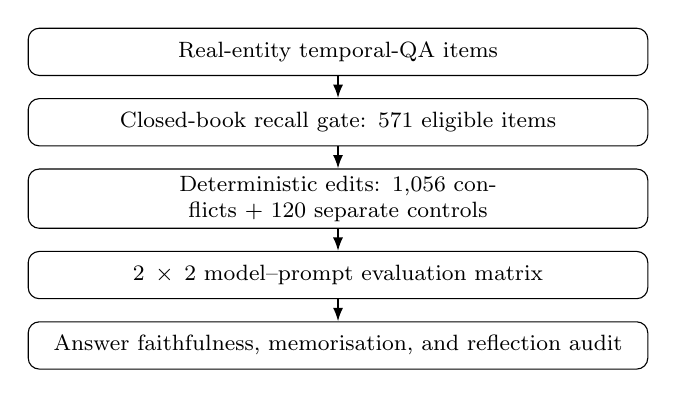
\begin{tikzpicture}[
  node distance=2.8mm,
  box/.style={draw, rounded corners, align=center, font=\footnotesize, text width=77mm, inner sep=2.4pt, minimum height=6mm},
  arr/.style={-{Latex[length=1.7mm]}, semithick}
]
\node[box] (n1) {Real-entity temporal-QA items};
\node[box, below=of n1] (n2) {Closed-book recall gate: 571 eligible items};
\node[box, below=of n2] (n3) {Deterministic edits: 1,056 conflicts $+$ 120 separate controls};
\node[box, below=of n3] (n4) {$2\times2$ model--prompt evaluation matrix};
\node[box, below=of n4] (n5) {Answer faithfulness, memorisation, and reflection audit};
\draw[arr] (n1)--(n2);
\draw[arr] (n2)--(n3);
\draw[arr] (n3)--(n4);
\draw[arr] (n4)--(n5);
\end{tikzpicture}
\caption{Context--Memory Conflict is an inference-only evaluation pipeline. Controls preserve the answer and are kept separate from genuine conflicts.}
\label{fig:pipeline}
\end{figure}

\subsection{Extension 2: Tennis-Domain Adaptation}

\paragraph{Dataset creation and processing.}
The tennis collection is synthetic and was created in two stages, documented in Appendix~\ref{app:tennis-prompts}. First, we used ChatGPT with \href{https://developers.openai.com/api/docs/models/gpt-5.5}{GPT-5.5} interactively to generate raw context--question--answer triples from scratch. A fragment of the raw-generation instruction was recovered, but the continuation, session export, complete batch history, exact model snapshot, and decoding settings are unavailable. Second, ChatGPT 5.5 received existing training examples together with their gold answers and generated supervised TISER reasoning, timeline, reflection, and answer traces. No external source corpus is recorded, so this description rests on our recollection rather than independently authenticated provenance. The dataset is released under \href{https://creativecommons.org/licenses/by/4.0/}{CC BY 4.0}; repository code is released under MIT.

The recorded processing pipeline audits the schema, assigns identifiers and rule-based categories, converts records to standard and TISER-compatible prompts, checks duplicates, and performs a category- and exact-duplicate-group-aware 70/10/20 split with seed~42. The three disjoint splits contain 785 training, 113 development, and 224 test examples and jointly cover all 1,122 records. Trace generation was restricted to the training split. Generated outputs were structurally validated, mechanically repaired when necessary, and merged. The conversion CLI's \texttt{reported} mode byte-reproduces the tracked files; strict-XML mode is reserved for new experiments.

\paragraph{Adaptation strategies.}
At 0.5B scale, we compare the vanilla model under standard and TISER prompts with a tennis-only adapter. At 7B scale, we first test direct transfer of the original TISER adapter and then continue LoRA training from that adapter on tennis traces. The evaluator retains TISER's output parser while adding tennis-specific normalization for rankings, minute durations, punctuation, and articles.

\section{Experimental Setup}
\label{sec:experimental-setup}

\subsection{Data and Evaluation}

After a 2,048-token filter, TISER training uses 54,488 examples. The test set has 19,214 in-domain examples and 2,800 ToT-semantic OOD examples. The conflict subset is constructed from 15,898 real-entity in-domain items and is evaluated on the 1,056 conflicts and 120 controls described above.

\subsection{Tennis Split and Trace Accounting}

The 785-record training split is the candidate pool for supervised trace creation; it is not itself the file used for optimization. It partitions exactly as $50+600+135=785$. Train positions 0--49 have valid traces from an initial pilot and support only pilot/smoke runs. Train positions 50--649 are the disjoint 600-record trace artifact used by both reported tennis adaptations. For positions 650--784, requests were prepared in batches 13--15 but no generated outputs are present, so those 135 examples could not be used as supervised trace targets. The repository therefore contains traces for 650 unique training records overall, but the reported models use only the 600-record full-run file.

The 113 development examples have no training traces and were never used for gradient updates; the repository preserves split-distribution diagnostics but no model predictions or performance metrics for them. The 224 test examples likewise have no training traces and never affect gradients. They were, however, used to evaluate every completed condition and to rank the 7B candidates. All full evaluations use the same 224 IDs in the same order. The complete 785-record split and the unused generation requests are retained because they document the deterministic 1,122-record partition and experiment lineage. Deleting them would not change training---the configurations already point directly to the 600-record file---but would erase pilot provenance, break trace-coverage reconstruction, and make the published splits incomplete.

\subsection{Tennis Semantic-Quality Audit}

Structural validity does not establish that a gold answer is uniquely entailed by its context. A deterministic, risk-focused AI-assisted audit reviewed 302 of the 785 training records: all 50 pilot records, 193 of the reported 600, and 59 of the ungenerated 135. Ten reviewed examples were flagged as wrong or underdetermined: none in the pilot, seven inside the reported training file, and three in the ungenerated tail. Thus at least $7/600=1.17\%$ of the actual training artifact has a known semantic concern, but 407 of its records did not receive this semantic review. Because the selection deliberately over-sampled higher-risk temporal categories, neither $7/600$ nor $10/302$ estimates the population error rate.

The historical adaptations remain valid as exploratory comparisons on a fixed, documented artifact: all compared adapters use the same training and evaluation definitions, and a small amount of label noise does not by itself invalidate training. However, the models must not be described as trained on a clean or fully validated dataset, and the effect of the flagged examples cannot be quantified without a corrected-data retraining or ablation. The development and test labels also lack exhaustive semantic adjudication, so reported metrics inherit that limitation. Historical files are kept immutable; any corrections should create a versioned dataset, regenerate affected traces, and produce new model results.

A complete replacement audit has been prepared as blinded file batches. Two independent passes review all 1,122 context--question--gold rows and all 650 available traces; disagreements and proposed corrections receive a third adjudication. Imports require exact source evidence, and completed decisions will produce versioned scoring views without altering the historical inputs. The audit is still in progress, so no partial rate or corrected score is reported. The model label observed in the UI does not identify a verifiable API snapshot, and human calibration is unavailable.

\subsection{Models, Training, and Decoding}

Table~\ref{tab:settings} consolidates the training hyperparameters. LoRA~\cite{hu2022lora} targets the $q$, $k$, $v$, and $o$ attention projections. The reproduction uses completion-only loss and no base-model quantization; the 7B continued-adaptation run loads the base in 4-bit precision. All reported answer generations are greedy. Reproduction and conflict runs allow up to 768 new tokens; tennis evaluation allows up to 768 tokens at 0.5B and 256 at 7B.

\begin{table}[t]
\centering
\caption{Hyperparameters for the reported trained adapters. Effective batch includes gradient accumulation.}
\label{tab:settings}
\setlength{\tabcolsep}{2.6pt}
{\footnotesize
\begin{tabular}{lcccccl}
\toprule
\textbf{Run} & \textbf{$n$} & \textbf{Ep.} & \textbf{LR} & \textbf{Batch} & \multicolumn{2}{c}{\textbf{LoRA}} \\
\cmidrule(lr){6-7}
& & & & & \textbf{$r/\alpha$} & \textbf{drop.} \\
\midrule
TISER 7B & 54{,}488 & 3 & $2{\times}10^{-4}$ & 16 & 16/32 & .05 \\
Tennis 0.5B & 600 & 1 & $2{\times}10^{-4}$ & 1 & 16/32 & .05 \\
Continued 7B & 600 & 2 & $2{\times}10^{-4}$ & 16 & 16/32 & .05 \\
\bottomrule
\end{tabular}
}
\end{table}

The reported continued-adaptation result is the highest-scoring condition in a grid over one to three epochs, learning rates $\{5{\times}10^{-5},1{\times}10^{-4},2{\times}10^{-4}\}$, and gradient accumulation $\{4,8\}$ with per-device batch size~4. All 22 distinct candidates were evaluated on the identical 224 examples, which makes their pairwise comparison fair. It does not make the winning score independent: once those outcomes are inspected and the maximum is selected, the set functions as validation data even though it never enters a gradient update. The winning condition leads two runners-up by one correct answer. The 0.732/0.856 result is therefore an exploratory selected estimate. With no preserved evidence of development-set model evaluation, the lowest-cost correction is to freeze this adapter and evaluate it once on the 113 records, without switching adapters afterward.

The implemented follow-up first compares the original adapter C0 and locked tennis winner C1 on a frozen seed-42 sample of up to 100 items per original-TISER split. A 10,000-resample paired interval for the five-split macro-EM difference triggers fresh C1R and R25 training only when its upper bound is below $-0.02$; a lower bound above $-0.02$ stops as non-inferior, and other intervals stop as inconclusive. If triggered, C1R and R25 both start from C0 and run for 74 updates under the same current environment; R25 adds 200 validated original-TISER training rows. A token-matched R25-T sensitivity run occurs only when R25 supervised-token exposure differs from C1R by more than 10\%. Final freezing requires the complete data and reflection audits. It then fixes all applicable adapters, prompts, parsers, metrics, populations, and hashes before one evaluation on the 113 tennis inputs and original-TISER complement. No outcome from those populations may reopen training or adapter selection.

\subsection{Conflict Sampling and Reflection Audit}

Closed-book recall uses five samples with temperature~0.7 and top-$p$~0.9; the subsequent run matrix uses one greedy decode per item. We use item-level bootstrap confidence intervals with 2,000 resamples and seed~42, plus paired McNemar tests for the two headline axes.

For TISER-prompt cells, a Claude-based judge reportedly read the persisted reflection and returned a structured conflict indicator, conflict category, and short rationale in windows of 100 records. The reported judge result is secondary evidence: the exact Claude model version, full judge prompt, and row-level audit CSVs are not preserved in the repository, preventing independent reproduction. The replacement is a new UI-mediated study rather than a retrospective reconstruction. Two isolated GPT-5.5-labelled Codex tasks receive only blinded reflection text under conservative rubrics, and a third task adjudicates disagreements. Exact file prompts, response bytes, hashes, labels, control false-positive rates, Wilson intervals, disagreement, unscorable rows, class breakdowns, and silent overrides are retained. The observed UI model label is recorded, while API snapshot and decoding details remain unknown. This replacement is in progress and must be complete before its values replace the historical aggregates; agreement between model judges does not supply human calibration.

\subsection{Compute and Software}

The reproduction was trained on one H200 SXM GPU in bf16 for approximately 6.5 hours. Test and conflict generation used vLLM on an H100 SXM GPU; the full 22,014-example evaluation took approximately 17 minutes. Reported versions were PyTorch~2.4.1/CUDA~12.4, Transformers~4.46.3, PEFT~0.13.2, and TRL~0.12.2 for reproduction, and vLLM~0.22.0 with PyTorch~2.11/CUDA~13.0 for accelerated inference.

\section{Results}

\subsection{Baseline Reproduction}

Table~\ref{tab:baseline} reports the full in-domain evaluation. Our macro-EM is 0.033 below the paper, while macro-F1 is 0.005 higher; the reproduction is therefore in a similar overall performance regime, but its error profile differs substantially on TGQA.

\begin{table}[t]
\centering
\caption{TISER reproduction on five in-domain splits. \emph{Paper} is the comparable Qwen2.5-7B+TISER result; ToT-semantic (OOD EM 0.381) is excluded from the macro.}
\label{tab:baseline}
\setlength{\tabcolsep}{3.7pt}
{\footnotesize
\begin{tabular}{lrcccc}
\toprule
& & \multicolumn{2}{c}{\textbf{Ours}} & \multicolumn{2}{c}{\textbf{Paper}} \\
\cmidrule(lr){3-4}\cmidrule(lr){5-6}
\textbf{Split} & \textbf{$n$} & \textbf{EM} & \textbf{F1} & \textbf{EM} & \textbf{F1} \\
\midrule
TGQA            & 3{,}316 & 0.571 & 0.870 & 0.845 & 0.942 \\
TempReason L2   & 5{,}397 & 0.907 & 0.929 & 0.855 & 0.875 \\
TempReason L3   & 4{,}426 & 0.961 & 0.974 & 0.915 & 0.949 \\
TimeQA easy     & 2{,}997 & 0.980 & 0.989 & 0.979 & 0.983 \\
TimeQA hard     & 3{,}078 & 0.970 & 0.981 & 0.961 & 0.972 \\
\midrule
\rowcolor{gray!18}
\textbf{Macro (5)} & 19{,}214 & \textbf{0.878} & \textbf{0.949} & 0.911 & 0.944 \\
\bottomrule
\end{tabular}
}
\end{table}

TGQA combines low EM (0.571) with much higher F1 (0.870), a pattern consistent with partially correct or differently formatted answers. The repository does not preserve the row-level annotations needed to substantiate a previously reported adjusted-accuracy estimate, so we omit that estimate rather than treating it as a reproducible result.

\subsection{Context--Memory Conflict}

Table~\ref{tab:conflict} makes the 1,056 genuine conflicts the primary population and reports the 120 controls separately. The TISER-trained model with the TISER prompt reaches faithful-EM 0.774, compared with 0.348 for the vanilla model under a standard prompt. Both interventions help: relative to the same-model standard prompt, TISER prompting adds 0.214; relative to vanilla weights under the same TISER prompt, TISER training adds 0.249.

\begin{table}[t]
\centering
\caption{Run matrix. Conflict metrics use only genuine conflicts ($n=1{,}056$); control EM is separate ($n=120$). $\Delta$EM is relative to base+standard on conflicts.}
\label{tab:conflict}
\setlength{\tabcolsep}{1.4pt}
{\footnotesize
\begin{tabular}{lccccc}
\toprule
\textbf{Condition} & \textbf{Faith-EM} & \textbf{Faith-F1} & \textbf{Mem-EM} & \textbf{$\Delta$EM} & \textbf{Ctrl.\ EM} \\
\midrule
Base + standard & 0.348 & 0.579 & 0.295 & --     & 0.658 \\
Base + TISER    & 0.525 & 0.718 & 0.228 & +0.176 & 0.883 \\
TISER + standard & 0.560 & 0.759 & 0.251 & +0.211 & 0.700 \\
\rowcolor{gray!18}
\textbf{TISER + TISER} & \textbf{0.774} & \textbf{0.914} & \textbf{0.153} & \textbf{+0.425} & \textbf{0.900} \\
\bottomrule
\end{tabular}
}
\end{table}

For continuity with the original aggregation, faithful-EM over conflicts \emph{plus} controls is 0.380, 0.561, 0.574, and 0.787 in table order. The previously reported rise from 0.380 to 0.787 therefore includes controls; the conflict-only comparison is 0.348 to 0.774. On all 1,176 constructed rows, the prompt-axis difference is +0.213 and the model-axis difference is +0.225; both paired McNemar tests give $p<10^{-40}$.

Figures~\ref{fig:conflict-matrix} and~\ref{fig:conflict-classes} separate the model--prompt comparison from the conflict-type analysis.

\begin{figure}[t]
\centering
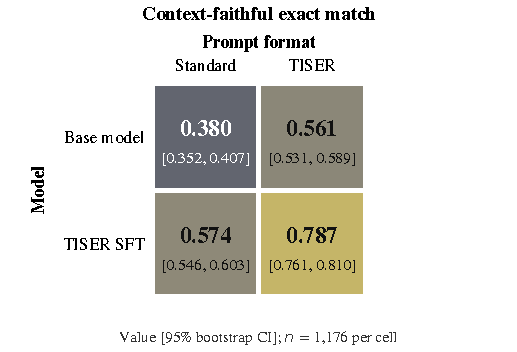
\includegraphics[width=\columnwidth]{figures/conflict_run_matrix.pdf}
\caption{Context-faithful exact match across the $2{\times}2$ model--prompt matrix. Each cell reports EM and its item-level bootstrap 95\% confidence interval over all 1,176 evaluation rows, including 120 answer-preserving controls. Both the TISER prompt and TISER fine-tuning improve faithfulness to the edited context.}
\label{fig:conflict-matrix}
\end{figure}

\subsection{Conflict Type and Reflection}

Table~\ref{tab:perclass} isolates the three genuine conflict types for the strongest condition. Date shifts and entity swaps are largely solved, but order reversal is a clear blind spot: it is the only class for which memorised EM exceeds faithful EM.

\begin{figure}[t]
\centering
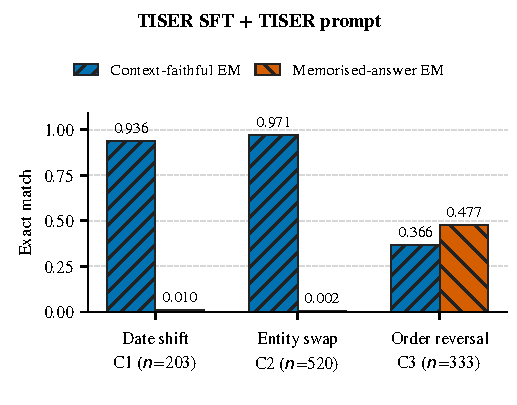
\includegraphics[width=\columnwidth]{figures/conflict_per_class.pdf}
\caption{Faithful and memorised-answer exact match for the TISER-fine-tuned model with the TISER prompt, shown only for the three genuine conflict classes (controls excluded). Date shifts and entity swaps are overwhelmingly resolved using the edited context; order reversals are the only class in which memorised-answer EM exceeds context-faithful EM.}
\label{fig:conflict-classes}
\end{figure}

\begin{table}[t]
\centering
\caption{Genuine-conflict results for TISER model+prompt. \emph{Refl.} is the secondary LLM-judge conflict-naming rate.}
\label{tab:perclass}
\setlength{\tabcolsep}{5.0pt}
{\footnotesize
\begin{tabular}{lrccc}
\toprule
\textbf{Class} & \textbf{$n$} & \textbf{Faith-EM} & \textbf{Mem-EM} & \textbf{Refl.} \\
\midrule
C1 date shift      & 203 & 0.936 & 0.010 & 0.020 \\
C2 entity swap     & 520 & 0.971 & 0.002 & 0.008 \\
\rowcolor{gray!18}
C3 order reversal  & 333 & 0.366 & 0.477 & 0.111 \\
\midrule
\textbf{All conflicts} & 1{,}056 & \textbf{0.774} & \textbf{0.153} & \textbf{0.043} \\
\bottomrule
\end{tabular}
}
\end{table}

The historical aggregate says that the reflection names the conflict in only 45/1,056 genuine conflicts (4.3\%) even though the final answer follows the edited context in 77.4\%. The corresponding control count is 4/120 (3.3\%). Their Wilson 95\% intervals are 3.2--5.7\% and 1.3--8.3\%, respectively, and a two-sided Fisher test gives $p\approx0.81$. Thus the preserved aggregates support the narrower conclusion that explicit flags were rare and concentrated in C3; they do not show discrimination above the control false-positive rate. The separate control arm reaches faithful-EM 0.900 in the strongest condition; because its answer equals memory by construction, it measures preservation of answerability rather than conflict resolution. A faithful answer without an explicit flag remains a descriptive silent override, not proof of an internal conflict-resolution mechanism.

\subsection{Tennis-Domain Adaptation}

Table~\ref{tab:tennis} reports all completed 224-example selection-set runs. At 0.5B, prompting alone does not help, while tennis-only training gives a modest gain. At 7B, the original TISER adapter transfers more strongly, and continued adaptation adds 0.152 EM and 0.155 F1. Isolation between adapter training runs prevents gradient leakage, but it does not prevent selection leakage: the 7B row is the maximum among 22 scores observed on these same records. It is therefore the best observed exploratory result rather than an unbiased final estimate.

\begin{table}[t]
\centering
\caption{Tennis temporal QA on the historically used selection set ($n=224$). Deltas are against the first row within each model-size block; \emph{Malformed} is an output count.}
\label{tab:tennis}
\setlength{\tabcolsep}{3.4pt}
{\footnotesize
\begin{tabular}{lccccc}
\toprule
\textbf{Condition} & \textbf{EM} & \textbf{F1} & \textbf{$\Delta$EM} & \textbf{$\Delta$F1} & \textbf{Malf.} \\
\midrule
\multicolumn{6}{l}{\emph{Qwen2.5-0.5B-Instruct}} \\
Base, standard prompt   & 0.379 & 0.472 & -- & -- & 0 \\
Base, TISER prompt      & 0.375 & 0.420 & $-$0.004 & $-$0.052 & 5 \\
\rowcolor{gray!10}
Tennis-only adapter     & 0.464 & 0.516 & +0.085 & +0.045 & 0 \\
\midrule
\multicolumn{6}{l}{\emph{Qwen2.5-7B-Instruct}} \\
Original TISER & 0.580 & 0.701 & -- & -- & 0 \\
\rowcolor{gray!18}
\textbf{Continued adaptation} & \textbf{0.732} & \textbf{0.856} & \textbf{+0.152} & \textbf{+0.155} & 0 \\
\bottomrule
\end{tabular}
}
\end{table}

\section{Discussion and Limitations}

The reproduction is strong overall but exposes the sensitivity of EM to answer formatting. More importantly, the two extensions answer different questions. The conflict probe shows that training and prompting can improve use of supplied evidence without making reflection an explicit contradiction detector. Tennis adaptation instead shows that the learned trace format transfers across domains and benefits from additional supervised examples, particularly at 7B scale.

Several limitations constrain these conclusions. The conflict set is restricted to facts the model already recalls confidently, so it is not a random sample of temporal questions. The reflection result relies on an unrecovered historical judge run; its aggregate rates are not independently reproducible, and the replacement audit has no human calibration. Greedy decoding provides one output per condition. For tennis, the creation process is reconstructed from project records rather than a complete session export, and the semantic/trace audit is unfinished. Seven known concerns occur inside the 600-record training artifact, whose size reflects an operational cutoff rather than a principled sample size. The best 7B setting was also selected on the 224-record evaluation split. Forgetting and the 113-record holdout result have not yet been measured, so the current tennis score remains exploratory. The team has no record of prior model-selection use of those 113 records, but the repository cannot exclude an unrecorded evaluation.

\section{Conclusion}

We reproduced TISER's strong in-domain temporal-QA performance and used two extensions to test complementary aspects of generalisation. Structured prompting and training made the model more willing to follow conflicting context, but its reflection rarely exposed the contradiction and remained weak on reversed event order. TISER also transferred to tennis narratives, where continued domain adaptation improved over direct transfer. Overall, following evidence, explaining a conflict, and adapting to a new domain are distinct capabilities and should be evaluated separately.

\section{Reproducibility}

The repository provides command-line workflows for data preparation, training, evaluation, scoring, auditing, and statistical analysis. Canonical configurations, seed~42, resolved run settings, predictions, metrics, and available environment metadata are preserved with the reported adapters and results. Dataset provenance, licences, recovered prompts, trace coverage, and semantic-review flags are documented separately. The offline audit supports blinded two-pass review and adjudication, while the Colab notebook runs the conditional retention, replay, and final-evaluation protocol with resumable predictions and training. Hashes bind each run to its source, data, configuration, adapter, and scoring view; no unexecuted value is presented as a result.

\clearpage
\onecolumn
\appendices

\section{Tennis Data-Generation Prompts}
\label{app:tennis-prompts}

The tennis data were created in two distinct stages. The following records preserve what can be supported about each stage; they are not presented as complete API logs.

\subsection{Stage 1: Raw Example Creation}

\begin{lstlisting}[style=prompt]
You are creating a synthetic domain-adaptation dataset for temporal reasoning in the professional tennis domain.

The dataset will be used to adapt a TISER-style temporal reasoning model. Your task is to generate RAW examples only.

For each example, output exactly one JSON object with these fields:

{
  "context": "...",
  "question": "...",
  "answer": "..."
}

Do NOT generate reasoning.
Do NOT generate timeline.
Do NOT generate reflection.
Do NOT add explanations.
Do NOT wrap the output in markdown.
Do NOT use code fences.

Return a JSON array containing exactly 50 examples.

GENERAL GOAL

Each example must test temporal reasoning in tennis match or tournament narratives.

The model should need to reason about the order, overlap, duration, or sequence of events. The answer must be inferable only from the context.

DOMAIN

Use professional tennis scenarios such as:

- match progression
- first set, second set, third set
- breaks of serve
- service holds
- tie-breaks
- set points
- match points
- rain delays
- roof closure
- medical timeouts
- injury treatment
- warm-up interruptions
- tournament rounds
- quarterfinals, semifinals, finals
- player withdrawals
- comebacks
- coaching violations
- crowd interruptions
- changeovers

You may use realistic player names such as Sinner, Alcaraz, Djokovic, Medvedev, Zverev, Rune, Rublev, Fritz, Nadal, Federer, Tsitsipas, Ruud, Shelton, De Minaur.

The events do NOT need to be historically true. Treat them as fictional but realistic tennis narratives.

CONTEXT REQUIREMENTS

Each context must:

- contain 3 to 6 sentences
- contain at least 3 temporal events
- be self-contained
- be unambiguous
- avoid external knowledge
- use natural sports-report language
- include clear temporal signals such as:
  - before
  - after
  - during
  - while
  - later
  - earlier
  - immediately after
  - at the same time
  - minutes later
  - in the first set
  - in the second set
  - before the tie-break
  - after the medical timeout

QUESTION REQUIREMENTS

Generate a balanced mix of question types:

1. Yes/No temporal comparison
Example:
"Did Sinner call the medical timeout before breaking serve?"

2. Which happened first?
Example:
"Which happened first: Alcaraz saved a break point or Medvedev won the tie-break?"

3. Which happened last?
Example:
"Which event happened last?"

4. What happened before X?
Example:
"What happened before the rain delay?"

5. What happened after X?
Example:
"What happened after Djokovic lost the second set?"

6. Duration / time gap
Example:
"How many minutes after the match started did the rain delay begin?"

7. During / overlap
Example:
"Was the roof being closed while the players were off court?"

8. Tournament progression
Example:
"Did Sinner reach the semifinal before playing the final?"

ANSWER REQUIREMENTS

Each answer must:

- be short
- be exact
- be unambiguous
- directly answer the question
- not include explanations

Use answer formats like:

- "Yes"
- "No"
- "Sinner broke serve"
- "The rain delay"
- "Alcaraz won the second set"
- "45 minutes"
- "The semifinal"

IMPORTANT BALANCE CONSTRAINTS

Among the 50 examples, approximately include:

- 15 Yes/No before-after questions
- 10 first/last ordering questions
- 8 what happened before/after questions
- 7 duration or time-gap questions
- 5 during/overlap questions
- 5 tournament progression questions

Difficulty distribution:

- 15 easy examples with direct before/after reasoning
- 25 medium examples with 3-4 ordered events
- 10 hard examples with 5-6 events or distractor events

QUALITY RULES

Avoid ambiguous cases such as:
- "in 2014" without month/day when asking about a specific month
- unclear transitions between teams, rounds, or sets
- answers that require real tennis knowledge
- questions with multiple valid answers
- contexts where two events could reasonably be interpreted in different orders

Do not repeat the same structure too many times.
Do not generate near-duplicate examples.
Do not always use the same players.
Do not always make the answer "Yes".
Use both positive and negative examples.

Before producing the final output, internally check each example:
- Is the answer derivable from the context?
- Is the temporal order clear?
- Is there only one correct answer?
- Is the answer short?
- Is the example about tennis?
- Did you avoid reasoning/timeline/reflection?

OUTPUT FORMAT

Return only a valid JSON array.

Example format:

[
  {
    "context": "Sinner held serve in the opening game. Djokovic called a medical timeout before Sinner broke serve in the fourth game. After the break of serve, rain delayed the match for twenty minutes.",
    "question": "Did Djokovic call the medical timeout before Sinner broke serve?",
    "answer": "Yes"
  },
  {
    "context": "Alcaraz saved two break points at 2-3 in the first set. Medvedev broke serve three games later. The set ended with Medvedev winning a tie-break.",
    "question": "Which happened first: Medvedev broke serve or Alcaraz saved two break points?",
    "answer": "Alcaraz saved two break points"
  }
]

Now generate exactly 50 examples.
\end{lstlisting}

We also recall constraints requiring contexts of approximately three to six sentences, at least three temporal events, balanced question types, varied difficulty, context-derivable answers, and exactly 50 valid JSON objects per requested batch, although we could not recover their exact wording. All 1,122 committed raw rows have exactly the three requested fields and three to five context sentences, which corroborates these recollections without authenticating the complete prompt. Because 1,122 is not divisible by 50, some aggregation, filtering, or partial-batch retention occurred; no surviving log resolves which.

\newpage
\subsection{Stage 2: TISER Trace Generation}

\begin{lstlisting}[style=prompt]
You will receive tennis temporal reasoning training examples.

For each example, generate only one JSONL record with the following fields:

{
  "question_id": "...",
  "output": "..."
}

The output must follow the TISER format:

<reasoning>
...
<timeline>
...
</timeline>
<reflection>
...
</reflection>
...
</reasoning>
<answer>GOLD_ANSWER</answer>

Rules:
- Use only information contained in the provided context.
- Reason explicitly about the temporal relations required to answer the question.
- Construct a chronological timeline containing the relevant events.
- In the reflection, verify that the reasoning and timeline support the gold answer.
- Do not invent events, dates, entities, or temporal relations.
- The final answer must match the provided gold_answer exactly.
- Preserve the question_id exactly.
- Output one JSON object per line.
- Output JSONL only. Do not include markdown, explanations, headings, or any additional text.
\end{lstlisting}

The requests also supplied \texttt{question\_id}, category, context, question, and gold answer. Generated rows contain \texttt{question\_id} and \texttt{output}. The final 600 records exactly match batches 1--12 in order. Nineteen malformed physical JSONL lines covering 26 records were recovered, and 200 outputs that lacked the requested XML-like tags were mechanically wrapped using their existing text and supplied gold answer. All 600 final rows pass structural and gold-answer-equality checks; those checks do not establish semantic entailment.

\begin{thebibliography}{00}

\bibitem{bazaga2025tiser}
A. Bazaga, R. Blloshmi, B. Byrne, and A. de Gispert,
"Learning to Reason Over Time: Timeline Self-Reflection for Improved Temporal Reasoning in Language Models,"
in \emph{Proceedings of ACL}, 2025.

\bibitem{xiong2024tgqa}
S. Xiong, A. Payani, R. Kompella, and F. Fekri,
"Large Language Models Can Learn Temporal Reasoning,"
in \emph{Proceedings of ACL}, 2024.

\bibitem{tan2023tempreason}
Q. Tan, H. T. Ng, and L. Bing,
"Towards Benchmarking and Improving the Temporal Reasoning Capability of Large Language Models,"
in \emph{Proceedings of ACL}, 2023.

\bibitem{chen2021timeqa}
W. Chen, X. Wang, and W. Y. Wang,
"A Dataset for Answering Time-Sensitive Questions,"
in \emph{NeurIPS Datasets and Benchmarks}, 2021.

\bibitem{hu2022lora}
E. J. Hu et al.,
"LoRA: Low-Rank Adaptation of Large Language Models,"
in \emph{International Conference on Learning Representations}, 2022.

\end{thebibliography}

\end{document}
